\documentclass[11pt,dvipdfmx]{ujarticle}
\usepackage{eee}
\usepackage{subfig}

\renewcommand{\labelenumi}{\alph{enumi}}
\renewcommand{\labelenumii}{\roman{enumii}}

\bibliography{3rd_power}
\begin{document}

\begin{jikkenTitle}
 \gakunen{3} 
 \numTitle{3}{総合負荷装置を用いた電力と力率の計測}
 \subTitle{\small{(Measurement of power and power factor by comprehensive load device)}} 
 \jikkenbi{令和04年06月23日(木)} 
 \jikkenbiII{令和04年06月30日(木)} 
 \kyoudou{3301 青木 柊人,3305 市川 潤} 
 \kyoudouII{3326 塚原 秀翔}
 \yoteibi{06/30}
 \yoteibiII{07/07}
 \yoteibiIII{07/14}
 \hanNumberName{1}{3309}{大山 主朗}
 \end{jikkenTitle}

\section{目的}
本実験では
\begin{itemize}
	\item 単相交流回路における電圧・電流・電力・力率を測定するための結線方法を学ぶ.
	\item 単相電力計と力率計の扱い方を習得する.
	\item 有効電力と力率,皮相電力と無効電力に関する理解を深める.
\end{itemize}
ことを目的とする.

\clearpage

\section{原理}
\subsection{磁気回路(Magnetic circuit)}
\wfig{hys:jikikairo}に示すように断面積$S\,[\mathrm{m}^2]$,平均磁路長$L\,[\mathrm{m}]$の鉄心に巻数$N_1\,[\mathrm{Turn}]$のコイルを巻き,これに$I\,[\mathrm{A}]$の電流を流すと,起磁力$N_1\cdot I\,[\mathrm{A}\cdot\mathrm{Turn}]$を生じる.
この起磁力により
\begin{equation}
	\phi = \frac{N_1\cdot I}{R_m}
\end{equation}
の磁束$\phi\,[\mathrm{Wb}]$を生じる.ここで$R_m$は以下に示す磁気抵抗である.
\begin{equation}
	R_m= \frac{L}{\mu_0 \mu_s S}
\end{equation}
ただし,$\mu_0 = 4\pi\times 10^{-7}\,\mathrm{F/m}$ は真空の透磁率であり,$\mu_s$は鉄心の比透磁率である.
ここで,磁路1\,mあたりの起磁力を磁化力$H\,[\mathrm{A/m}]$という. 磁化力$H$は
\begin{equation}
	H=\frac{N_1\cdot I}{L}
\end{equation}
である.また磁路断面積 1\,m$^2$あたりの磁束を,磁束密度$B\,[\mathrm{Wb/m}^2]$という.
\begin{equation}
	B=\frac{\phi}{S}
	\label{eq:hys:BphiS}
\end{equation}
ここで,$S\,[\mathrm{m}^2]$は磁路断面積を示す.
\begin{figure}[htbp]
	\centering
	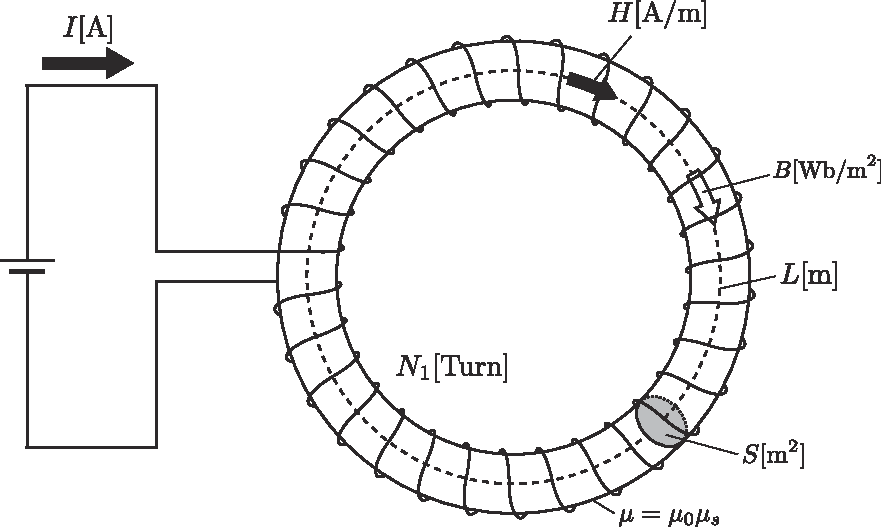
\includegraphics[width=70mm]{fig/magnetism_circuit.pdf}
	\caption{磁気回路}
	\label{fig:hys:jikikairo}
\end{figure}

鉄心の磁化力$H$と磁束密度$B$との関係を示す曲線をB-H曲線といい,一般に\wfig{hys:bhcurve}(a)のような飽和特性になる.
また磁化力$H$を正負の方向に増減すると,\wfig{hys:bhcurve}(b)の様なヒステリシス曲線(Hysteresis curve)になる.
\begin{figure}[htbp]
	\centering
	\begin{tabular}{cc}
		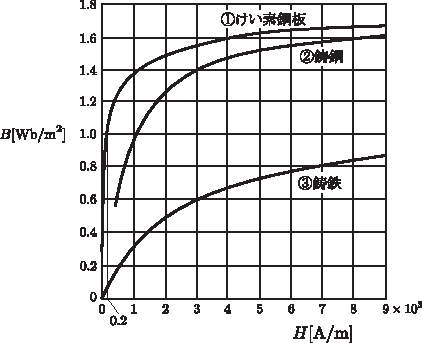
\includegraphics[width=70mm]{fig/bhcurve.pdf} &
		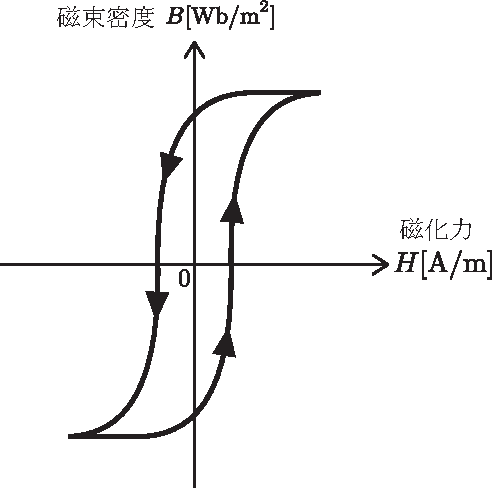
\includegraphics[width=70mm]{fig/hysteresis.pdf} \\
		(a) B-H 曲線 & (b) ヒステリシス曲線
	\end{tabular}
	\caption{B-H曲線とヒステリシス曲線}
	\label{fig:hys:bhcurve}
\end{figure}

\subsection{交流磁化特性}
\label{zika}
\wfig{hys:transformer}の変圧器のように,鉄心に巻かれた巻数$N_1$のコイルに交流電圧$V_1$を加えると,鉄心中に交番磁束$\dot{\phi}$を作るための電流(励磁電流)$i_0$が流れる.このとき磁束密度$B$と磁化力$H$との間にはヒステリシス特性があるため,励磁電流は\wfig{hys:hizumi}のようにひずみを生ずる.この現象を逆に利用して,励磁電流$i_0$と交番磁束$\dot{\phi}$の波形をなんらかの方法で取り出し,オシロスコープのX軸に励磁電流$i_0$の波形,Y軸に交番磁束$\dot{\phi}$の波形を入力すれば,オシロスコープの画面に鉄心のヒステリシス特性(B-H曲線)が描かれる.
\begin{figure}[htbp]
	\centering
	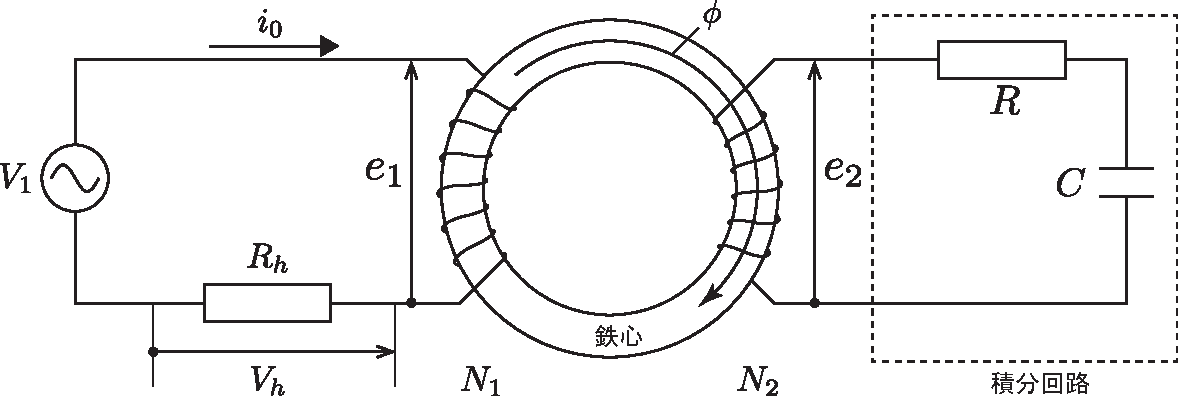
\includegraphics[width=140mm]{fig/transformer.pdf}
	\caption{変圧器の交流磁化特性測定回路}
	\label{fig:hys:transformer}
\end{figure}

励磁電流$i_0$の波形を直接取り出すのは難しいので,\wfig{hys:transformer}において励磁電流$i_0$が抵抗$R_h$を流れるときの電圧変化,すなわち
\begin{equation}
	V_h = i_0R_h
\end{equation}
として取り出す.また,交番磁束$\dot{\phi}$は次の様にして取り出す.

\wfig{hys:transformer}において二次巻線$N_2$と鎖交する磁束の時間に対する変化が二次誘起電圧$e_2$として現れるため
\begin{equation}
	e_2 = -N_2\frac{d \phi}{dt}
	\label{eq:hys:e2}
\end{equation}
となり,\weq{hys:e2}を変形すると
\begin{equation}
	d \phi = \frac{1}{N_2}\times e_2\times dt
	\label{eq:hys:dphi}
\end{equation}
となるから,交番磁束$\phi$は\weq{hys:dphi}を積分すれば求まることとなる.すなわち,二次巻線に発生する電圧$e_2$を時間で積分すればよい.そこで二次側にCR積分回路を接続しコンデンサCの両端から$e_2$を積分した,交番磁束に比例した電圧をとりだす.

\begin{figure}[h]
  \begin{minipage}[c]{0.5\hsize}
    \centering
    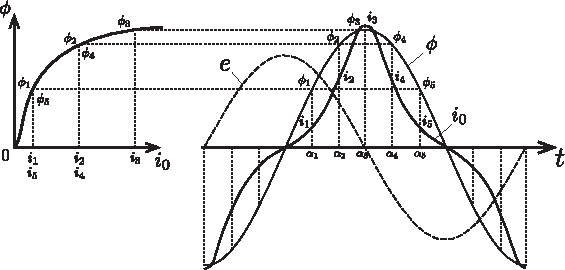
\includegraphics[scale=1.2]{fig/hizumi_a.pdf} 
    \caption{ヒステリシス現象のない場合}
  \end{minipage}\\
  \begin{minipage}[c]{0.5\hsize}
    \centering
    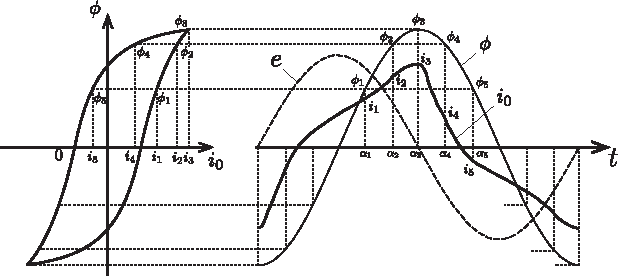
\includegraphics[scale=1.2]{fig/hizumi_b.pdf}
    \caption{ヒステリシス現象のある場合}
  \end{minipage}
  \centering
  \caption{ヒステリシス現象}
   \label{fig:hys:hizumi}
\end{figure}

\subsection{磁区}
\subsection{理想変圧器}
\subsection{実際の変圧器}
\subsection{磁気飽和現象}\label{hohwa}
\subsection{抵抗損と漂遊負荷損\cite{1130282271832577152}}
ブリッジ法などで測定した巻線の抵抗(直線抵抗)を$r_{d}$とし,巻線に流れる交流電流を$I$とすると,抵抗損は$I^{2}r_{d}$である.しかし,実際の損失はこの値より大きくなる.その理由は次の2つである.
\begin{enumerate}[(1)]
	\item \textbf{導体内のうず電流損}\\
	電流による漏れ磁束が導体自身の断面に鎖交するため,導体内にうず電流が発生し,電流密度が不均一になり,導体断面積が減少したのと同じ結果となり抵抗が増加する.またその増加分は$5 \sim 20\,\%$である.また,うず電流は抵抗に反比例するため,巻線の断面積が大きい場合はうず電流を低減することができる\cite{11302822718325772}\cite{1130282270467697152}.
	\item \textbf{構造材料内の損失}\\
	漏れ磁束の一部は,タンクの側板,締め付けボルトなどを通るため,それらの部分にうず電流損失やヒステリシス損失が生じる.以上の2つを合わせて漂遊負荷損といい,抵抗損の$5 \sim 20\,\%$になる.
	抵抗損と漂遊負荷損の和が負荷損であるが,その値はほとんど電流の2乗に比例する.すなわち,二次負荷電流を$I_{2}$とすれば負荷損$W_{l}$は
	\begin{equation}
		W_{l}=I_{2}^{2}r
	\end{equation}
	で表される.
\end{enumerate}

\subsection{積分回路}
\subsection{電流密度}

\clearpage
\section{方法}
\subsection{使用器具}
今回の実験で使用した器具を\wtab{kigu}に示す.
\begin{table}[h]
\centering
\caption{使用器具}
\label{tab:kigu}
\begin{tabular}{ccclc}
\hline
装置名     & 製造会社     & 型番             & \multicolumn{1}{c}{定格}        & 製造番号       \\ \hline
電力計     & YOKOGAWA & B-5038.H1.2/2  & レンジ:120-240V, 5-25A           & 632        \\
低力率用電力計 & YOKOGAWA & B-3041         & レンジ:120-240V, 1-5A            & 04823M     \\
交流用電圧計  & YOKOGAWA & B-3039.44.9/10 & レンジ:0.1-300V                  & 70-1       \\
交流用電流計  & YOKOGAWA & B-2044.45.1/7  & レンジ:1-5A                      & OG 0575    \\
力率計     & YOKOGAWA & B-2054.49.1/1  & \multicolumn{1}{c}{120V}      & L94-004318 \\
スライダック  & 東芝       & B-5091.H1.2/3  & \multicolumn{1}{c}{0-130V}    & 625        \\
総合負荷装置  & 山菱電機株式会社 & UL-100-30      & \multicolumn{1}{c}{100V, 30A} & L94-004164 \\ \hline
\end{tabular}
\end{table}

\subsection{実験手順}
\begin{enumerate}[a)]
\item 電力計によるRL負荷の電力測定
\label{RLhuka}
\begin{enumerate}[(1)]
	\item \wfig{circ}のように回路を構築する.\footnote{電源線をはずして作業を行う}
	\begin{figure}[h]
	\centering
	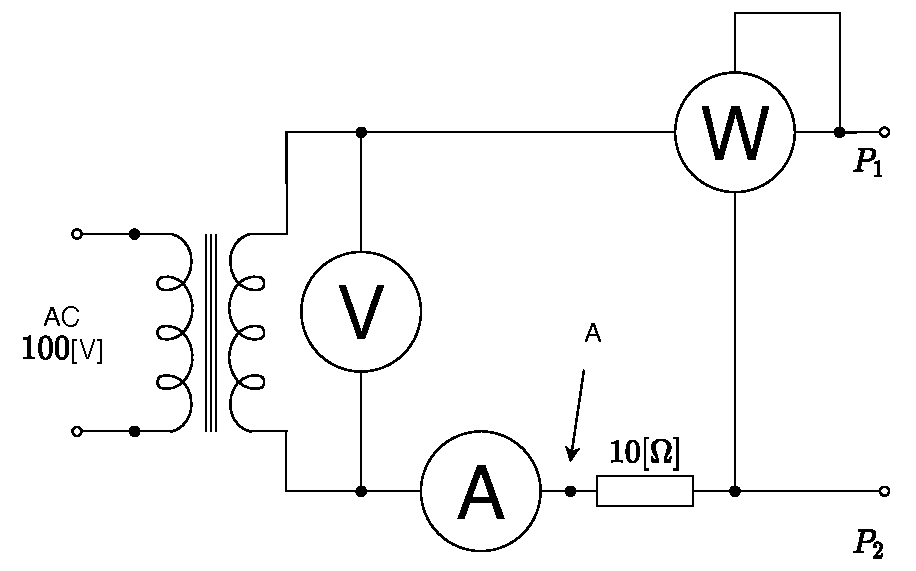
\includegraphics[scale=1]{./fig/circ.pdf}
	\caption{測定回路}
	\label{fig:circ}
\end{figure}
\item スイッチS1を開き,負荷の電流調節つまみをDEC方向いっぱいに回した.\footnote{DEC:decreaseの略で減らすの意.この処理は負荷に電流を加えないための初期設定}
\item スイッチS2を$X_{L}$側にし,リアクタンスとしてLを選択.\label{S2}
\item 力率を1に設定(負荷を$R=1.0, X=1.0$に設定)
\item S1を閉じ,商用電源の電圧(スライダック部)が$100\,\rm{V}$になるように調整し,総合負荷装置の電源ランプの点灯を確認した.
\item 電流計の読みが$1\,\rm{A}(\pm 0.1\,\rm{A})$となるようにSL1で電流を調整し,電力,力率,電圧,電流を計測し,表を作成.

この際,計算力率は\weq{calfac},皮相電力は\weq{calpo}で求めた.
\begin{align}
	\cos \theta' &=\frac{P_{a}}{VI}
	\label{eq:calfac}\\
	P&=VI
	\label{eq:calpo}
\end{align}
\item 電流を$2\,\rm{A}$から$5\,\rm{A}$まで$1\,\rm{A}$刻みで同様の計測を実施.
\item 力率を以下のように設定し,上記の計測を繰り返した.
\begin{itemize}
	\item 力率0.8 ($R=0.8,\quad X=0.8$)
	\item 力率0.6 ($R=0.6,\quad X=0.6$)
	\item 力率0.4 ($R=0.4,\quad X=0.4$)
	\item 力率0.2 ($R=0.2,\quad X=0.2$)
\end{itemize}
\end{enumerate}
\item 電力計によるRC負荷の電力測定
\begin{enumerate}[(1)]
	\item \ref{RLhuka}を参考にし,\ref{S2}の部分でリアクタンスとしてCを選択した.(スイッチS2を$X_{C}$側に設定)
\end{enumerate}
\item 低力率用電力計による電力計測
\begin{enumerate}[(1)]
	\item \wfig{circ}において,電力計を低力率用のものに変更.
	\item 力率0.2 ($R=0.2,\quad X=0.2$)に設定し\ref{RLhuka}と同様の計測を行った.
\end{enumerate}
\end{enumerate}
\clearpage

\section{結果}
\begin{itemize}
	\item 入力電圧-励磁電流-電力-電力の関係は\wtab{re1}のようになった.入力電圧上昇とともに電流,電力,位相の増加が確認できる.
	\begin{table}[h]
	\centering
	\caption{励磁電流特性}
	\label{tab:re1}
	\begin{tabular}{cccc}
	\hline
	入力電圧$V\,[\rm{V}]$& 電流$i_{0}\,[\rm{A}]$& 電力$P_{0}\,[\rm{W}]$& 位相\,[\rm{deg}]  \\ 
	\hline
	75  & 0.307    & 1.84     & 85.41643 \\
	80  & 0.337    & 2.10      & 85.53252 \\
	85  & 0.378    & 2.36     & 85.78774 \\
	90  & 0.429    & 2.64     & 86.07928 \\
	95  & 0.483    & 2.96     & 86.30133 \\
	100 & 0.552    & 3.34     & 86.53107 \\ \hline
	\end{tabular}
	\end{table}
\end{itemize}
\clearpage

\section{考察}
\subsection{課題考察}
\begin{enumerate}[1.]
	\item 変圧器の励磁電流について調べ,なぜ流れ,どのような役割をしているのかを考察せよ.\cite{1130282270091029760}
	
	実際の変圧器では,一次・二次巻線には抵抗があるため,負荷電流が流れると銅損が生じる.
	また,鉄心の透磁率は無限大ではないため,磁束$\dot{\phi}$をつくるために電流が必要となる.
	この電流を励磁電流(exciting current)という.
	これによって,鉄心中には鉄損が生じる.
	\item 励磁電流がひずみ波形になる理由を説明せよ.
	
	実際の変圧器では,一次巻線に交流電圧を加えると,鉄心の磁気飽和現象(参考:\ref{hohwa})やヒステリシス現象(参考:\ref{zika})が生じるため,励磁電流は非正弦波交流(ひずみ波形)となる\cite{1130282270091029760}.
	\item 磁性材料のヒステリシス損失について調査せよ.特に使用電圧が変化したとき及び使用電圧の周波数が変化したときについてそれぞれ説明せよ.\cite{11302822718577152}
	\label{hlos}
	
	ヒステリシス損は,鉄心内の磁束が方向及び大きさを変化することにより鉄心を構成する磁気分子が方向・配列を変え,分子相互間に摩擦損が生じることに起因するもの.
	また,ヒステリシスループの囲む面積に比例する.従って,周波数に比例し,さらに,最大磁束$\Phi_{m}$のとき磁束密度$B_{m}$がほぼ$1\,\rm{T}$以下では$B_{m}^{1.6}$に比例し,$1\,\rm{T}$以上では$B_{m}^{2}$に比例する.
	普通,$B_{m}=1 \sim 1.8\,\rm{T}$で使用されるため,鉄心の単位質量当たりのヒステリシス損$\omega_{h}$は以下で与えられる.
	\begin{equation}
		\omega_{h}=\sigma_{h}fB_{m}^{2}=k_{1}\frac{E^{2}}{f}\,[\rm{W/kg}]
		\label{eq:he}
	\end{equation}
	ここで,$\sigma_{h}$はヒステリシス損係数,$f\,[\rm{Hz}]$は周波数,$B_{m}\,[\rm{T}]$は最大磁束$\Phi_{m}$のときの鉄心磁束密度,$k_{1}$は比例定数,$E\,[\rm{V}]$は誘導起電力である.\\
	\weq{he}より使用電圧及び使用電圧の周波数が増加すると損失も増加することがわかる.
	\item 磁性材料のうず電流損について調査せよ.特に使用電圧が変化したとき及び使用電圧の周波数が変化したときについてそれぞれ説明せよ.\cite{11302822718577152}
	\label{uzu}
	
	うず電流損は,磁束の変化によって鉄心内に起電力を生じ,電流が流れる結果,抵抗損失が生じるもので,鋼板の厚さ,周波数及び磁束密度のそれぞれ2乗に比例する.
	これらより,単位重量当たりのうず電流損$\omega_{e}$は次式で与えられる.
	\begin{equation}
	\omega_{e}=\sigma_{e}t^{2}f^{2}B_{m}^{2}=k_{2}t^{2}E^{2}\,[\rm{W/kg}]
	\label{eq:uzue}
	\end{equation}
	ここで,$\sigma_{e}$はうず電流損係数,$t\,[\rm{mm}]$は積層鋼板1枚の厚さ,$k_{2}$は比例定数である.\\
	この\weq{uzue}より使用電圧及び使用電圧の周波数が増加すると損失も増加することがわかる.
	\item 電力計を使用して測定するときの損失とヒステリシス曲線から求めた損失について比較検討し考察せよ.\label{pi}
	
	ヒステリシス損は\ref{hlos}で述べたようにヒステリシスループ内の面積に比例し,\weq{w}を用いて算出することができる.
	なお,ヒステリシスループ内の面積はImageJを用いて算出した.
	また,保存したヒステリシスループの波形は$1\,\rm{DIV}=1\,\rm{cm}$となるように加工をしたため,$[\rm{cm^{2}}]=[\rm{DIV^{2}}]$である.
	\begin{align}
	W_{h}\,[\rm{W}]&=f\times A \times S\times L \times 換算\rm{X}軸測定条件\,[\rm{A/m\cdot 1/DIV}]\times 換算\rm{Y}軸測定条件\,[\rm{Wb/m^{2}\cdot 1/DIV}]\nonumber\\
	\label{eq:w}
	\end{align}
	ここで$A=3.84\times 10^{-4}\,\rm{m^{2}}$は鉄心断面積,$S\,[\rm{cm^{2}}]$は計測したヒステリシスループ内面積,$L=0.122\,\rm{m}$は平均磁路長である.また,実験地は東京であるため$f=50\,\rm{Hz}$である.
	また,$80\,\rm{V}, 100\,\rm{V}$の各場合について測定した損失(\wtab{re1}参照)と\weq{w}を用いて計算により算出した損失を\wtab{los}に示す.
	さらに,測定誤差として$P_{0}$と$W_{h}$の差を求めた.
	
	\begin{table}[h]
	\centering
	\caption{測定損失と計算損失}
	\label{tab:los}
	\begin{tabular}{ccccc}
	\hline
	入力電圧$V\,[\rm{V}]$ & ループ内面積$S\,[\rm{DIV}]$ & 測定損失$P_{0}\,[\rm{W}]$ & 計算損失$W_{h}\,[\rm{W}]$&損失誤差$\,[\rm{W}]$ \\ \hline
	80   & 5.61   & 2.10 & 1.99& 0.11\\
	100  & 8.10   & 3.34 & 2.88 &0.46\\ \hline
	\end{tabular}
	\end{table}
	
	どちらの場合においても測定損失の方が計算損失より大きいことがわかる.
	これは理想の変圧器では考慮していないことがあるからである.(\ref{real}参照)
	
	また,入力電圧が上昇すると損失及び計算値と実際の値の差(誤差)も増えることがわかり,これは上の考察\ref{uzu}, \ref{pi}とも一致する.
	\item 変圧器の鉄心用珪素鋼板について調べよ.\cite{1130282270091060}
	
	変圧器の鉄心には,飽和磁束密度と透磁率が大きく,鉄損の少ない電磁鋼板が用いられる.電磁鋼板は,ヒステリシス損を減少させるためケイ素を$4.5\,\%$程度含有させている.
	電磁鋼板には一方だけ磁束を通しやすい性質の材料もある.また,1枚1枚の電磁鋼板の表面に施してある絶縁皮膜が.温度上昇の一因となるうず電流が流れるのを防ぐ働きをしている.
\end{enumerate}

\subsection{独自考察}
\begin{enumerate}[1.]
	\item 理想変圧器とは以下の条件を満たす変圧器のことをいう\cite{1130000795154912128}.
\begin{itemize}
	\item 巻線の抵抗が0である.
	\item 鉄心の透磁率が無限大であり,したがって磁気回路における磁気抵抗が0である.
	\item 鉄心の鉄損が0である.
	\item 鉄心の磁気飽和は無視できる.
\end{itemize}
\item 一方,実際の変圧器は理想変圧器と異なり,以下のことを考慮しなければならない
\label{real}
\cite{1130154912128}.
\begin{itemize}
	\item 一次及び二次巻線の抵抗や漏れリアクタンスが存在する.
	\item 主磁束を作るために起磁力,すなわち励磁電流が必要である.
	\item 鉄心中に鉄損が存在する.
	\item 鉄心の磁気飽和を無視することは実際上できないが,ここでは特に考慮しない.
\end{itemize}
\item 損失は大きく分けて,コアに発生する鉄損,コイル巻線(誘導機の場合は二次導体も含む)に発生する銅損,そして,摩擦や空気抵抗に起因する機械損に分類できる.
さらに,負荷によって導体,鉄に生じる損失のうち鉄損,銅損に含まれないものを漂遊負荷損と呼ぶ.
これらをまとめたものを\wfig{loss_analysis}に示す.
\begin{figure}[h]
	\centering
	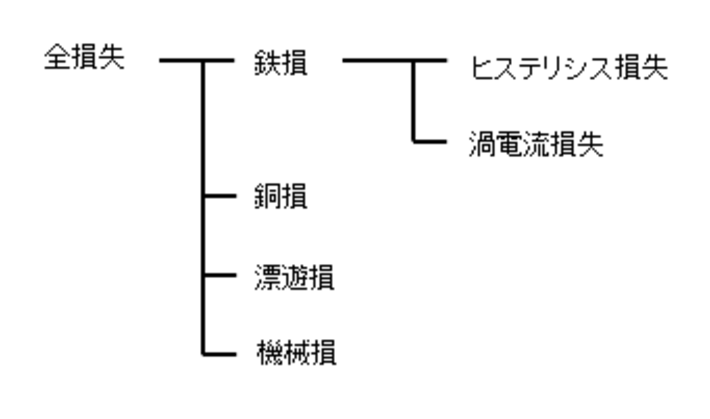
\includegraphics[scale=0.8]{./fig/loss_analysis.pdf}
	\caption{\cite{fdls}}
	\label{fig:loss_analysis}
\end{figure}
\end{enumerate}

\clearpage
\section{結論}
本実験を通して
\begin{itemize}
	\item 単相交流回路における電力・電流・電圧・力率の測定方法
	\item 単相電力計及び力率計の使用方法
	\item 電力に関する諸知識
\end{itemize}
を習得することができた.

\newpage
\printbibliography[title=参考文献]

\end{document}